\chapter{Validação e Resultados}

Nesse capítulo será apresentado o processo de validação e análise do projeto
desenvolvido nessa proposta. A validação foi divida em 2 etapas, a primeira
foi a validação via software, por meio de simulações e ferramentas de teste,
e a segunda foi a validação via hardware, onde foi produzido sistemas embarcados
protótipos para teste do protocolo no mundo real. Nas seções a seguir esse
trabalho irá entrar detalhes no que foi feito em cada etapa e quais foram
os resultados obtidos.

\section{Simulações e Testes Unitários}

O desenvolvimento dos códigos desse projeto seguiu a metodologia \textit{Test Driven Development}
a qual determina que a medida em que os módulos de um sistema vão sendo desenvolvidos, é desenvolvido
em paralelo também as suas próprias rotinas de testes. Tais testes podem ser divididos em categorias
como \textit{teste de integração}, onde é testado a integração entre diferentes módulos, e como o
\textit{teste unitário}, onde é testado o modulo como um caixa preta fora do sistema. Pare isso,
existem hoje em dia várias \textit{frameworks} que ajudam o desenvolvedor nesse processo,
nesse trabalho foi utilizada a framework \textit{CppUTest}, uma framework voltada para
testes unitários em projetos de sistemas embarcados.

Um teste unitário é nada mais do que rotinas de testes que são escritas em código e que
interagem com os módulos desenvolvidos e testam se, dependendo da entrada, foi produzido
a saída esperada. Nas figuras \ref{fig:test-queue} e \ref{fig:test-memmgr} a seguir é possível
visualizar exemplos dessas rotinas de testes.

\begin{figure}[H]
    \centering
	\caption{Teste das funcionalidades do modulo Circular Queue}
    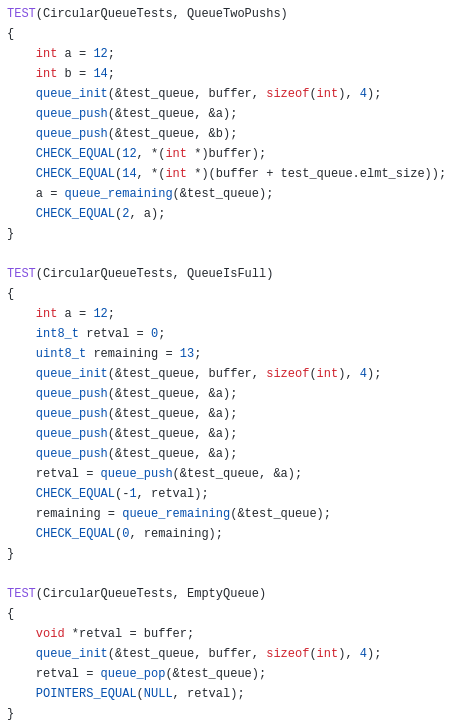
\includegraphics[height=0.75\textheight,keepaspectratio]{img/test-queue.png}
    \label{fig:test-queue}
    
    Fonte: Autor, 2022.
\end{figure}

\begin{figure}[H]
    \centering
	\caption{Teste das funcionalidades de alocação do modulo Memory Manager}
    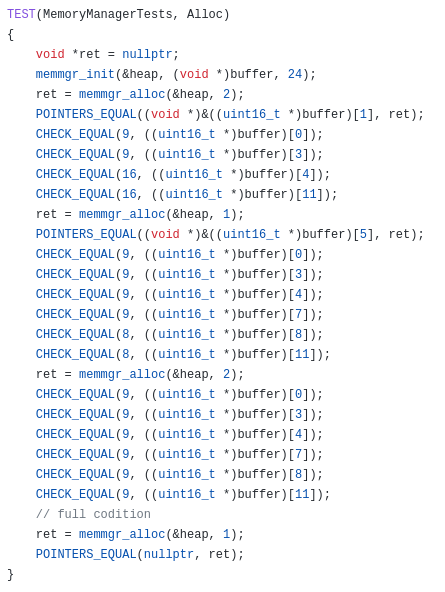
\includegraphics[height=0.62\textheight,keepaspectratio]{img/test-memmgr.png}
    \label{fig:test-memmgr}
    
    Fonte: Autor, 2022.
\end{figure}

\subsection{Testes Unitários como Simuladores}

Uma possibilidade que os testes unitários fornecem é a de simular fluxos do protocolo.
Ao ver todo o modulo do projeto como uma caixa preta, podemos entender que na
sua entrada vamos ter diferentes tipos de pacotes que serão processados seguindo
alguma lógica definida internamente e na sua saída um outro pacote como resposta deste
estimulo de entrada. Seguindo essa logica, foi desenvolvido testes para cada fluxo
proposto nesse projeto. Na figura \ref{fig:test-gw} a seguir podemos ver uma trecho
de um dos testes para validar o fluxo de conexão com o gateway.

\begin{figure}[H]
    \centering
	\caption{Teste de fluxo de conexão de nó com gateway}
    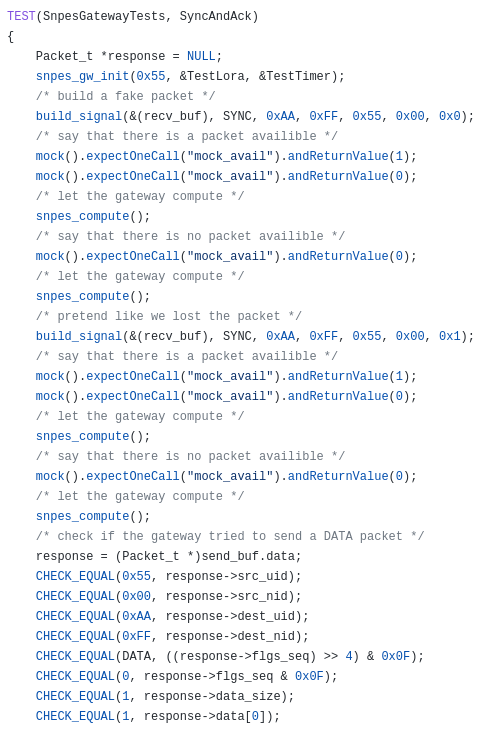
\includegraphics[width=0.75\textwidth,keepaspectratio]{img/test-gw.png}
    \label{fig:test-gw}
    
    Fonte: Autor, 2022.
\end{figure}

\subsection{Resultado dos Testes Unitários}

Foram desenvolvidas 41 rotinas de testes totalizando 525 verificações afim
de validar todos as funcionalidades de cada modulo do sistema como também
simular o sistema como um todo para todos os fluxos propostos nesse trabalho.
É interessante observar que, como mostra na figura \ref{fig:langs} a seguir
e também na tabela \ref{tab:files}, aproximadamente metade de todo código 
produzido no projeto foi para testes, que foram exclusivamente escritos em C++.

\begin{figure}[H]
    \centering
	\caption{Percentual das linguagens presentes no projeto}
    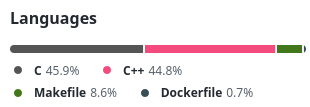
\includegraphics[height=0.11\textheight,keepaspectratio]{img/langs.png}
    \label{fig:langs}
    
    Fonte: Autor, 2022.
\end{figure}

Na figura \ref{fig:tests} a seguir é possível ver o resultado dos testes desenvolvidos,
onde todos passaram com sucesso.

\begin{figure}[H]
    \centering
	\caption{Execução dos testes desenvolvidos}
    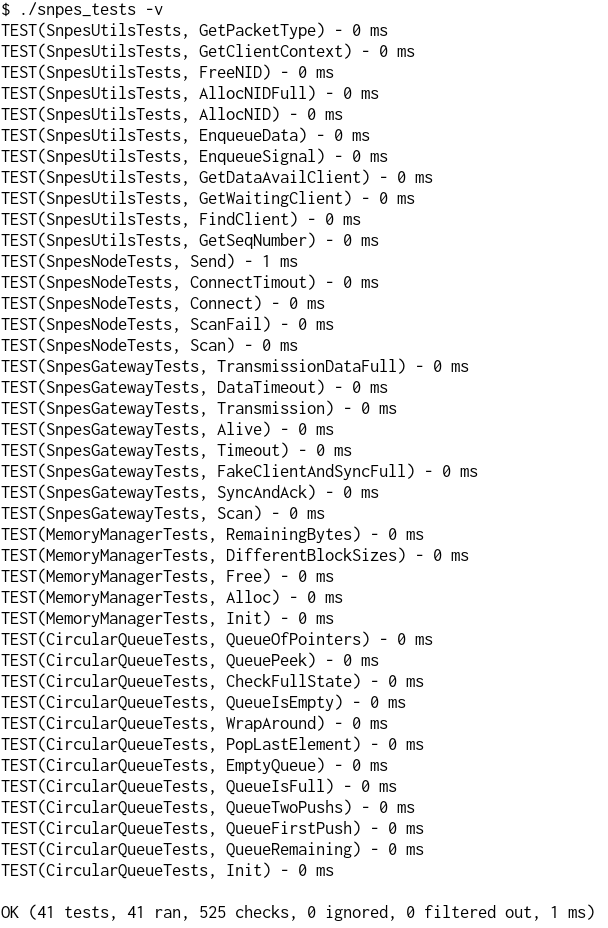
\includegraphics[height=0.57\textheight,keepaspectratio]{img/tests.png}
    \label{fig:tests}
    
    Fonte: Autor, 2022.
\end{figure}

\newpage

\subsection{Cobertura do código}

Além das APIs de testes, a framework \textit{CppUTest} oferece a geração de
\textit{relatórios de cobertura}. Esses relatórios descrevem a porcentagem de
linhas de código de cada arquivo fonte que foram testadas. Além disso ele
gera também um descrição de quantas vezes qualquer linha de código do projeto
foi executada e quais não foram. Na figura \ref{fig:cov} a seguir é possível
visualizar o resultado de cobertura do projeto.

\begin{figure}[H]
    \centering
	\caption{Relatório de cobertura do projeto}
    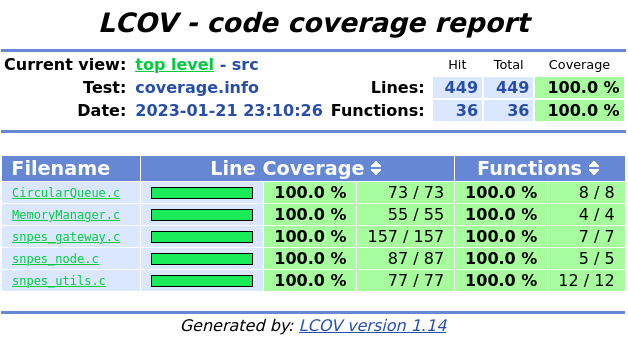
\includegraphics[height=0.225\textheight,keepaspectratio]{img/cov.png}
    \label{fig:cov}
    
    Fonte: Autor, 2023.
\end{figure}

Como é visto na figura a cima o projeto teve 100\% de cobertura no código,
ou seja, todas as linhas programadas foram executadas pelo menos uma vez.

\section{Protótipos e Testes em Campo}

Nesta etapa é apresentado os protótipos de hardware construídos para da validação da proposta
no mundo real, o objetivo é construir dispositivos Nó e um dispositivo
Gateway para fazer testes práticos e estudar como o protocolo proposto se comporta
em determinados cenários.
Na figura \ref{fig:prototipo} a seguir mostra o esquemático definido para os protótipos.

\begin{figure}[H]
    \centering
	\caption{Esquema do Protótipo de teste e validação}
    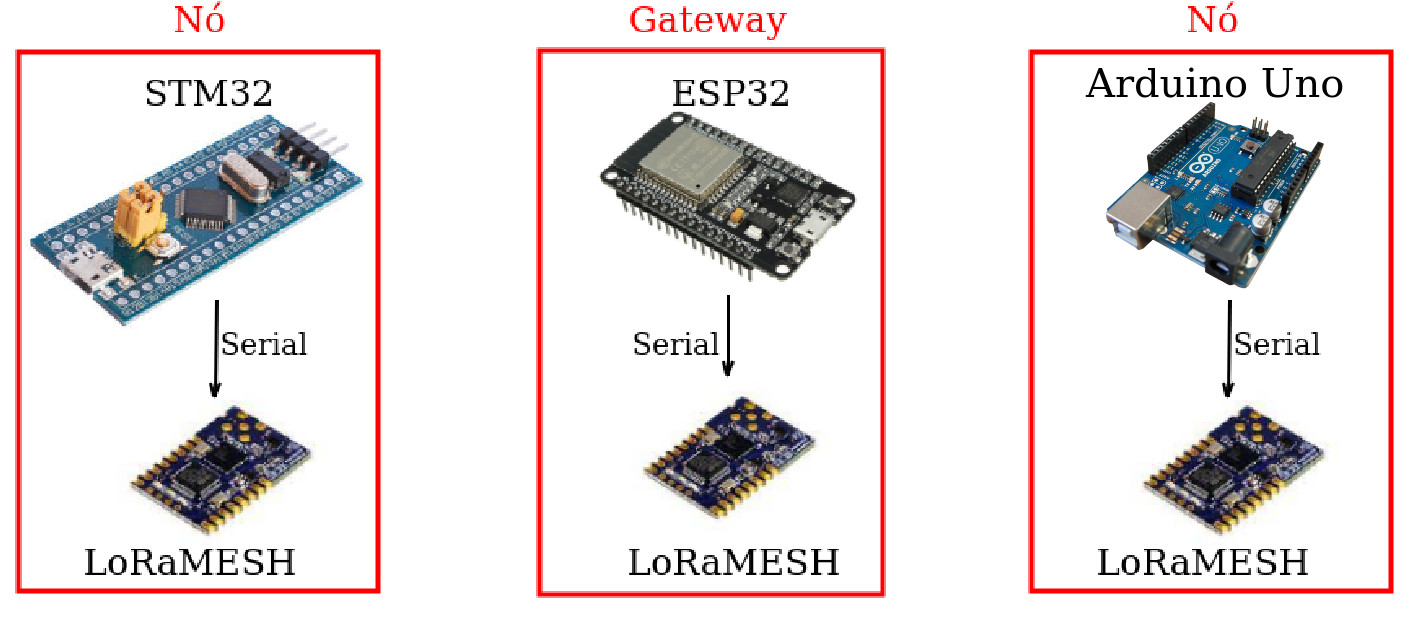
\includegraphics[height=0.21\textheight,keepaspectratio]{img/prop.jpg}
    \label{fig:prototipo}
    
    Fonte: Autor, 2022.
\end{figure}

\newpage

Foram escolhidos os microcontroladores STM32F1 "Blue Pill", o ESP32 Dev Kit,
e o Arduino Uno
por serem opções populares atualmente no cenário de IoT, mas também por serem
arquiteturas completamente diferentes. Dessa forma, é possível validar o nível
de portabilidade do protocolo e das interfaces definidas no desenvolvimento. O
objetivo é que não precise refatorar nada já implementado, e assim, os
microcontroladores rodem exatamente o mesmo código escrito em C. Já para o
Radio LoRa, foi escolhido o Radioenge LoRaMESH, uma opção que estava disponível
para uso no laboratório de pesquisa de sistemas embarcados do Centro de Informática.

\subsection{Driver do Rádio LoRa}

O Rádio periférico LoRaMESH desenvolvido pela Radioenge implementa as funcionalidades
LoRa em hardware, para envio e recebimento de mensagens o
rádio oferece uma interface serial documentada no site da Radioenge. Afim de
facilitar a vida do desenvolvedor, a Radioenge oferece um driver de código aberto
que abstrai os comandos usados na serial em forma de uma API, porém, esse driver
foi desenvolvido para Arduino e em seu código possui funções dependentes do
hardware. Dessa maneira, para garantir a modularização dos componentes de software
de acordo com o diagrama de blocos definido no capítulo anterior, e reforçado na Figura
\ref{fig:lora-driver} a seguir, foi necessário substituir as funções de leitura
e escrita na serial usadas nesse driver por uma Interface Serial, para que dessa forma,
ele possa ser o mesmo para as 3 arquiteturas escolhidas.

\begin{figure}[H]
    \centering
	\caption{Modularização do Driver LoRa da Proposta}
    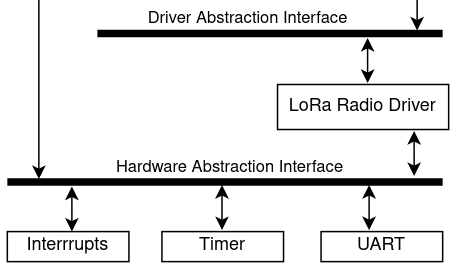
\includegraphics[width=0.45\textwidth,keepaspectratio]{img/lora-driver.png}
    \label{fig:lora-driver}
    
    Fonte: Autor, 2022.
\end{figure}

Mais uma vez, uma das grandes vantagens dessa arquitetura definida na proposta é que o
projeto não está dependente ao hardware, se por alguma razão se troque de rádio
LoRa, basta em teoria trocar o driver de acordo com a imagem a cima,
e dessa forma o projeto continua funcional sem necessidade de nenhuma refatoração.

\newpage

\subsection{Protótipos finais}

Na Figura \ref{fig:prop-final} a seguir pode ser visto a montagem final dos protótipos
que foram utilizados para os testes em campo.
da esquerda para a direita encontra-se o STM32F1 "Blue Pill", o ESP32 Dev Kit,
e o Arduino Uno, cada um conectado ao seu rádio LoRaMESH da Radioenge.

\begin{figure}[H]
    \centering
	\caption{Protótipos construídos}
    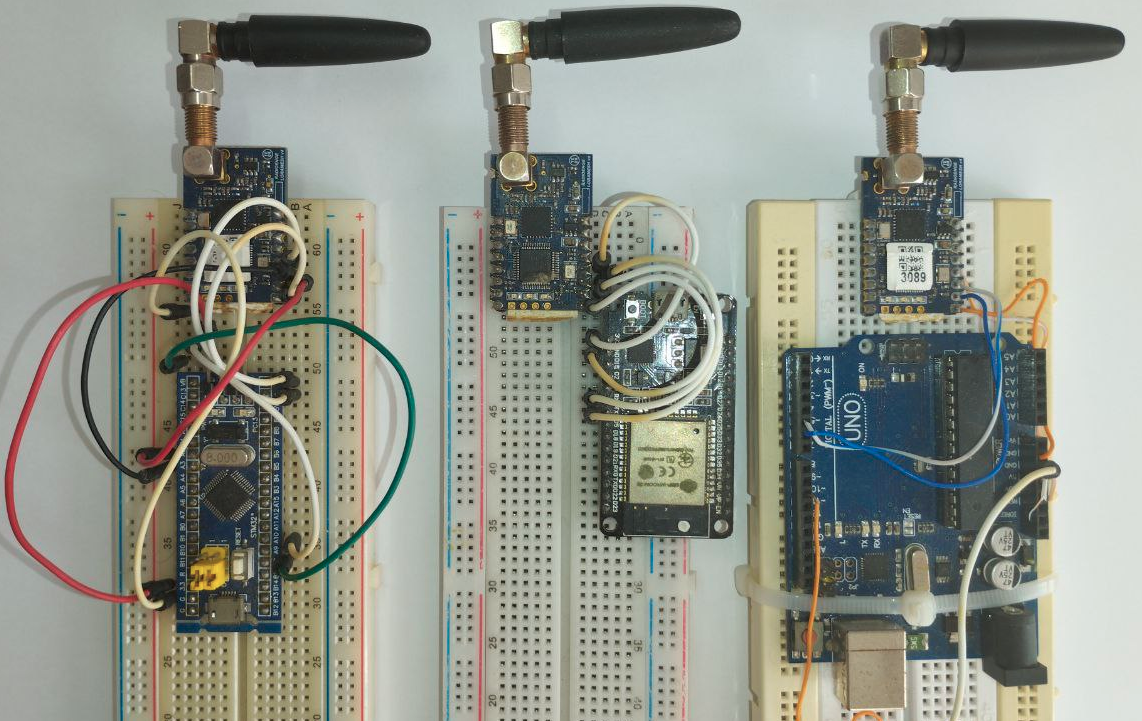
\includegraphics[width=0.49\textwidth,keepaspectratio]{img/prop-final.png}
    \label{fig:prop-final}
    
    Fonte: Autor, 2022.
\end{figure}

\subsection{Preparação para os testes}

Os testes em campo foram divididos em duas categorias: curtas distâncias
e longas distâncias. Para cada uma foi usado uma diferente configuração
nos rádios. Na figura \ref{fig:lora-config} a seguir é possível ver um resumo
das configurações existentes para o rádio LoRaMESH da Radioenge.

\begin{figure}[H]
    \centering
	\caption{Tabelas de configuração do Rádio LoRaMESH}
    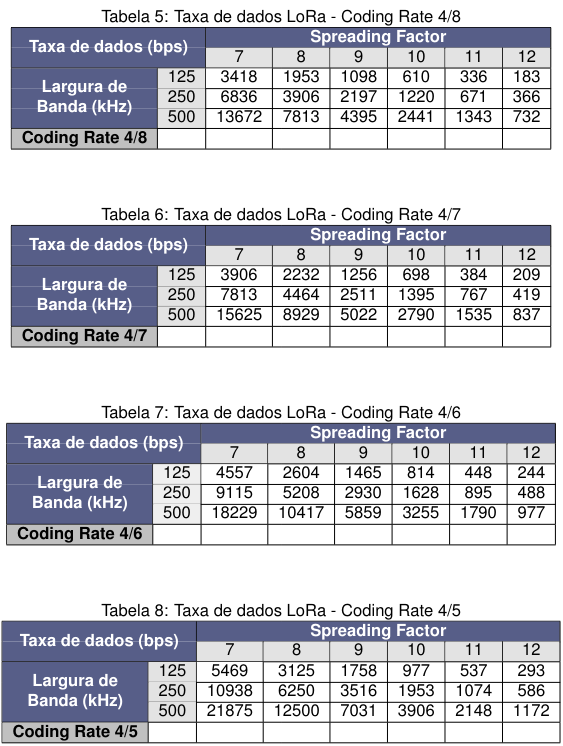
\includegraphics[width=0.4\textwidth,keepaspectratio]{img/lora-config.png}
    \label{fig:lora-config}
    
    Fonte: Radioenge, 2022.
\end{figure}

\newpage

As configurações usadas nos testes para cada uma das categorias podem ser vistas na
tabela \ref{tab:config} a seguir.

\begin{longtable}{|l|l|l|l|}
    \caption{Configuração usada para os testes}\label{tab:config}\\
    \hline
    \textbf{Categoria} & \textbf{Coding Rate} & \textbf{Largura de Banda} & \textbf{Spreading Factor} \\
    \hline
    Curtas distâncias & 4/8 & 250kHz & 7 \\
    \hline
    Longas distâncias & 4/8 & 250kHz & 12 \\
    \hline
\end{longtable}

\subsubsection{Cenários de testes}

Foi escolhido 3 cenários de testes para campo:
\begin{enumerate}
    \item varredura de gateways na área de alcance.
        \begin{itemize}
            \item Objetivo: avaliar se o gateway será encontrado pelos nós.
        \end{itemize}
	\item múltiplas conexões simultâneas no gateway.
         \begin{itemize}
            \item Objetivo: avaliar se o gateway será capaz de aceitar e manter múltiplas conexões.
        \end{itemize}
	\item transmissão continua de dados para o gateway.
        \begin{itemize}
            \item Objetivo: avaliar a porcentagem de transmissões bem e mal sucedidas dentro
            de um determinado período como também avaliar de todas transmissões bem sucedidas
            quantos por cento delas tiveram que em algum momento retransmitir algum pacote.
        \end{itemize}
\end{enumerate}

Todos esses cenários foram executados aproximadamente na máxima distância em que
os rádios ainda eram capazes de trocarem entre si o menor sinal possível. Essas distâncias
foram encontradas empiricamente para cada categoria definida a cima. Ao descobrir
essas distâncias foi montado os seguintes esquemas físicos das figuras \ref{fig:short-final}
e \ref{fig:long-final}.

\begin{figure}[H]
    \centering
	\caption{Esquema físico dos testes a curtas distâncias}
    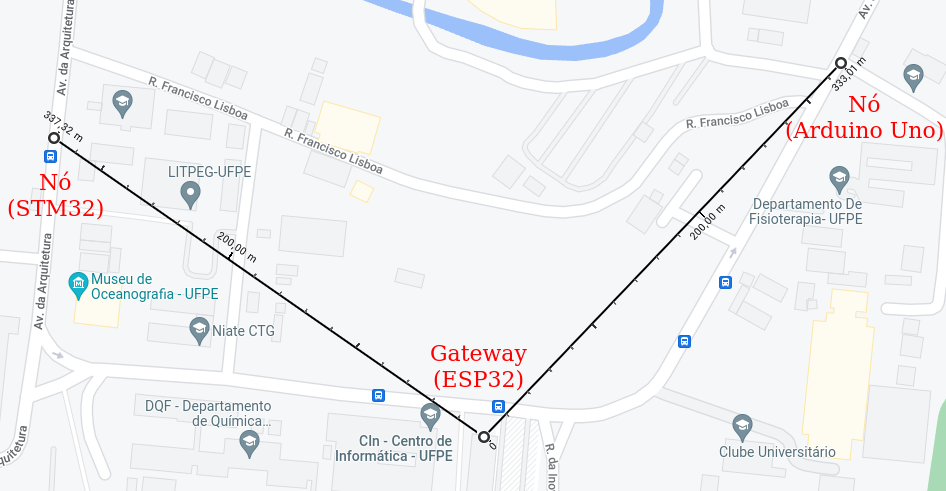
\includegraphics[width=0.8\textwidth,keepaspectratio]{img/short-final.png}
    \label{fig:short-final}
    
    Fonte: Autor, 2022.
\end{figure}

\newpage

A distância média para a categoria de curtas distâncias foi por volta de 350m ponto
a ponto, com isso foi montado o cenário que pode ser visto na figura \ref{fig:short-final} a cima.

\begin{figure}[H]
    \centering
	\caption{Esquema físico dos testes a longas distâncias}
    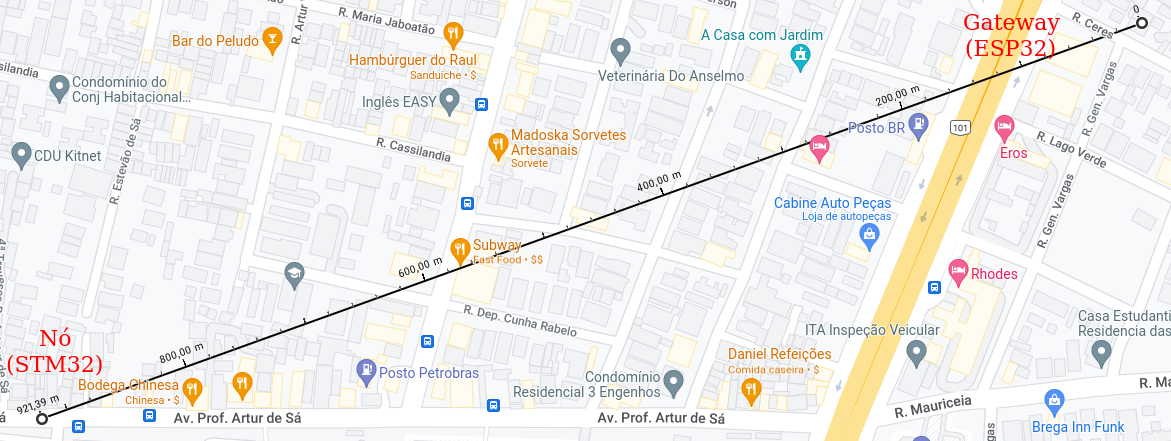
\includegraphics[width=\textwidth,keepaspectratio]{img/long-final.png}
    \label{fig:long-final}
    
    Fonte: Autor, 2022.
\end{figure}

Já para a categoria de longas distâncias a comprimento máximo ponto a ponto foi por volta de 950m,
e assim foi montado o cenário que pode ser visto na figura \ref{fig:long-final} a cima.

\subsection{Resultados dos Testes em Campo}

\subsubsection{Teste de Varredura de Gateways na Área de Alcance}

O teste de varredura é relativamente simples já que consiste apenas do envio de alguns
pequenos pacotes descritos fluxos do capítulo anterior. Esse teste não apresentou nenhum
problema para as duas categorias e os gateways foram encontrados pelos nós onde
o pior tempo registrado foi de aproximadamente 1200 mili segundos na categoria de longas
distâncias. Apesar da simplicidade, é importante salientar que apesar de simples esse fluxo
é extramente necessário já que os nós podem apenas se conectar a qualquer gateway
se souberem seu UID, com isso a varredura auxilia ao nós descobrirem UIDs de gateways
na sua área de alcance.

\subsubsection{Teste de Conexões simultâneas}

O teste de conexões simultâneas também é relativamente simples e consiste em verificar
se o gateway aceita mais conexões após um Nó já ter previamente conectado, se ele
distribui os NIDs corretos para as novas conexões, e se ele é capaz de gerenciar
essas conexões simultaneamente. O teste foi bem sucedido para todas a categorias
e também foi validado a tentativa de conexões com o gateway a aproximadamente ao mesmo tempo,
ou seja, os dois nós solicitaram conexão ao gateway praticamente iguais, e gateway
executou os fluxos de conexão em paralelo com cada um dos nós.

\newpage

\subsubsection{Teste de transmissões simultâneas continuas em curta distância}

O teste de transmissão simultânea e continua consiste em, após conectados ao gateway, cada
Nó irá frequentemente solicitar e transmitir uma quantidade fixa de 20 bytes para o gateway.
A frequência dessas transmissões foi configurada para a cada 3 segundos no Nó do STM32
e a cada 6 segundos para o Nó do Arduino, afim de gerar casos onde os dois Nós tentaram
transmitir ao mesmo tempo e com isso o gateway terá que paralelizar essas transmissões.
Na tabela \ref{tab:result-short} é possível visualizar os resultados obtidos. É importante
ressaltar que as porcentagens a seguir foram geradas no firmware do Gateway, com isso
ele avalia as transmissões dos dois nós como um todo.

\begin{longtable}{|l|l|}
    \caption{Resultados: Transmissão simultânea e continua -- Curtas Distâncias}\label{tab:result-short}\\
    \hline
    \textbf{Categoria} & Curtas distâncias \\
    \hline
    \textbf{Duração do Teste} & 60 minutos \\
    \hline
    \textbf{Transmissão bem sucedidas} & 91\% \\
    \hline
    \textbf{Transmissão mal sucedidas} & 9\% \\
    \hline
    \textbf{Retransmissão de pacotes dos envios bem sucedidos} & 33\% \\
    \hline
\end{longtable}

Com isso é possível observar que de todas as transmissões apenas 9\% falharam, e também,
dentre as transmissões bem sucedidas, aproximadamente 2/3 não precisaram retransmitir nenhum
pacote.

\subsubsection{Teste de transmissão continua a longas distâncias}

Já na categoria de longas distâncias foi utilizado apenas o Nó da STM32, mas o teste
ainda consiste de solicitação e envio continuo de 20 bytes na frequência definida anteriormente.
Os resultados podem ser vistos na tabela \ref{tab:result-long} a seguir.

\begin{longtable}{|l|l|}
    \caption{Resultados: Transmissão continua -- Longas Distâncias}\label{tab:result-long}\\
    \hline
    \textbf{Categoria} & Longas distâncias \\
    \hline
    \textbf{Duração do Teste} & 30 minutos \\
    \hline
    \textbf{Transmissão bem sucedidas} & 58\% \\
    \hline
    \textbf{Transmissão mal sucedidas} & 42\% \\
    \hline
    \textbf{Retransmissão de pacotes dos envios bem sucedidos} & 98\% \\
    \hline
\end{longtable}

É possível notar que dessa vez tivemos um resultado extramente diferente do anterior.
A taxa de falhas foi relativamente alta a 42\% e mais interessante ainda é a porcentagem
de retransmissão de pacotes nos envios bem sucedidos, o que mostra que praticamente todos
os pacotes precisaram ser retransmitidos.

\subsection{Footprint final do protocolo}

Foi também gerado um relatório de \textit{footprint} para analisar o custo da implementação
desse protocolo no firmware de cada microcontrolador usado. Esses relatórios podem ser vistos
nas figuras \ref{fig:foot-ard}, \ref{fig:foot-stm} e \ref{fig:foot-esp} a seguir.

\begin{figure}[H]
    \centering
	\caption{Footprint do projeto no Arduino Uno}
    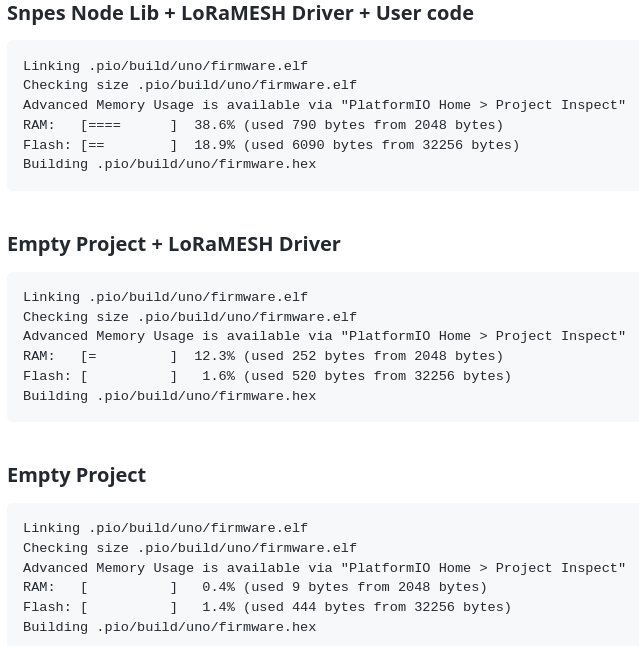
\includegraphics[width=0.85\textwidth,keepaspectratio]{img/foot-ard.png}
    \label{fig:foot-ard}
    
    Fonte: Autor, 2022.
\end{figure}

Da figura \ref{fig:foot-ard} é possível destacar que a biblioteca do protocolo
para o Nó no Arduino Uno ocupou aproximadamente de 538 bytes da memória RAM, e
5570 bytes da memória Flash. Em porcentagem representam respectivamente 26.3\%
e 17.3\% de cada. Um resultado aceitável considerando todas as funcionalidades
do protocolo e que o Arduino Uno é um
microcontrolador embarcado com poucos recursos comparados a outros, porém,
ainda sim o protocolo se mostrou eficiente com os recursos de hardware o que
é um ponto extremamente positivo pois esses recursos precisam ser dedicados
o máximo possível aos desenvolvedores do sistema final.

\newpage

\begin{figure}[H]
    \centering
	\caption{Footprint do projeto no STM32F1}
    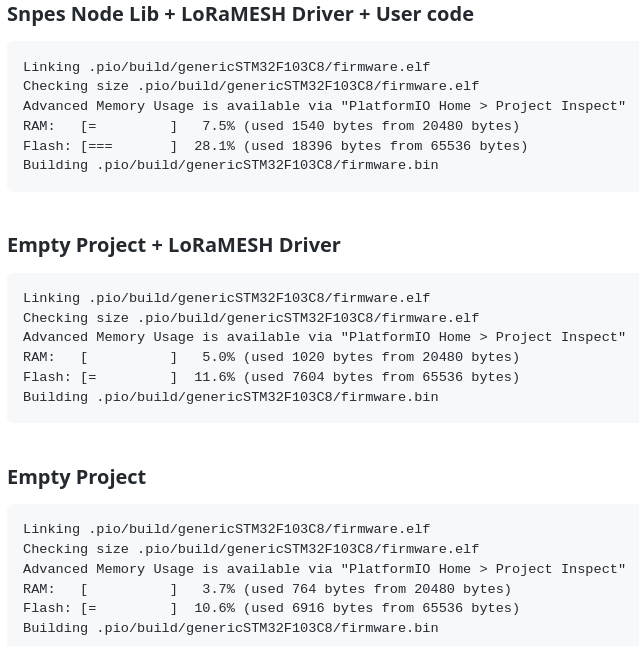
\includegraphics[width=0.85\textwidth,keepaspectratio]{img/foot-stm.png}
    \label{fig:foot-stm}
    
    Fonte: Autor, 2022.
\end{figure}

Agora figura \ref{fig:foot-stm} é possível visualizar que a biblioteca do protocolo
para o Nó no STM32F1 ocupou aproximadamente de 520 bytes da memória RAM o que se
mostra muito próximo ao visto no Arduino Uno e que é o esperado. Na memoria Flash
foi usado 10792 bytes quase o dobro do visto no Arduino Uno, que provavelmente
se deve em consideração por serem arquiteturas diferentes e assim as instruções
quando compiladas terão diferentes tamanhos e quantidades. Em porcentagem 
representam respectivamente 2.5\%
e 16.5\% de cada. Um resultado, mais uma vez, muito positivo, principalmente
no footprint da memória RAM, pelos fatos levantados anteriormente.

\begin{figure}[H]
    \centering
	\caption{Footprint do projeto no ESP32}
    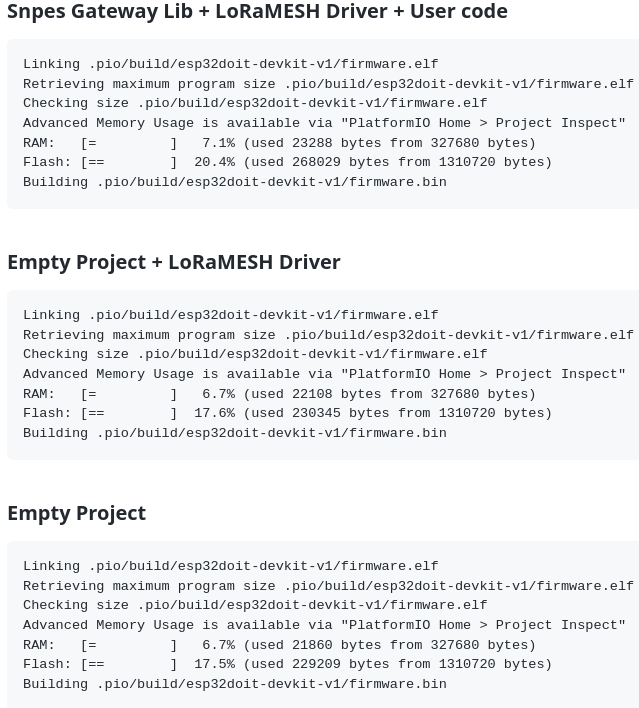
\includegraphics[width=0.85\textwidth,keepaspectratio]{img/foot-esp.png}
    \label{fig:foot-esp}
    
    Fonte: Autor, 2022.
\end{figure}

E por fim, na ESP32 podemos analisar o footprint da biblioteca do protocolo 
para o modo Gateway, que como foi destacado no capítulo anterior, sua implementação
é bem mais custosa pois exige a criação de grandes \textit{buffers} para gerencias
múltiplas conexões e transmissões. Pela figura \ref{fig:foot-esp} podemos ver que
a biblioteca ocupou aproximadamente 1180 bytes que memória RAM, bem mais do que
a biblioteca do Nó o que é realmente esperado. Na memória Flash foi usado 37684
bytes. Em porcentagem representam respectivamente 0.4\% e 2.8\% de cada.
Um resultado muito positivo mas muito interessante de destacar que, mesmo com toda
a necessidade de mais recursos de hardware para o caso do gateway, ainda sim para
o ESP32 o impacto foi muito pouco significativo, isso se da pela quantidade extramente
grande de memória RAM e Flash encontradas nesse microcontrolador.

\newpage